\documentclass[aspectratio=169]{beamer}
\setbeamertemplate{navigation symbols}{}
  
%\usetheme{Stuttgart}

%\useinnertheme{circles}

%\usepackage{ngerman}
%\usepackage{media9}
\usepackage{array}
%\newcolumntype{x}[1]{>{\centering\arraybackslash}p{#1}}
\usepackage{amsmath,bm}
\usepackage{amssymb}
\usepackage{mathtools}
\usepackage{accents}
\usepackage{graphicx}
\usepackage{hyperref}
%\usepackage{multirow}

%benedict
%\usepackage{tikz}
%\usetikzlibrary{arrows,calc,decorations.pathmorphing}
%\usetikzlibrary{decorations.pathreplacing}


\setbeamertemplate{navigation symbols}{}
%\setbeamertemplate{footline}[frame number]


  
  
\setlength{\leftmargini}{0pt}
\setlength{\leftmarginii}{5pt}
\setlength{\leftmarginiii}{10pt}
%\beamersetuncovermixins{\opaqueness<1>{25}}{\opaqueness<2->{15}}



\definecolor{iagcolor}{RGB}{36,128,200}
\definecolor{lightgrey}{RGB}{130,130,130}
\setbeamerfont{exampleblock}{size=\footnotesize}
\newcommand{\textc}[1]{\textcolor{iagcolor}{#1}}
\newcommand{\textcc}[1]{\textcolor{red}{#1}}
\newcommand{\tgray}[1]{\textcolor{lightgray}{#1}}
\newcommand\dd[2]{\frac{d #1}{d #2}}
\newcommand\ddp[2]{\frac{\partial #1}{\partial #2}}
\newcommand\lc{\left (}
\newcommand\rc{\right )}

\newcommand{\thet}{\vartheta}  
  


  
%GVEC SLIDES
%\usepackage[all, cmtip]{xy} % needed for commutative diagrams

\setbeamertemplate{footline}{%
  \raisebox{3pt}{\makebox[\paperwidth]{\makebox[20pt]{\textcolor{gray}{
  \textbf{F.Hindenlang},
  \textit{Analysis of the BIEST vacuum field solver, implementing the Merkel approach}
  \hspace{0.3\textwidth} \insertframenumber }}}}} 
  
\begin{document}

\title{Analysis of the BIEST vacuum field solver, implementing the Merkel approach}
 \author{ Florian Hindenlang$^{\,1}$}
 \date{ } 
 \institute{$^1$Numerical Methods division (NMPP), IPP Garching }


% \logo{%\raggedright\includegraphics[width=0.44\textwidth]{eurofusion.pdf}\hspace{2.5cm}
%       \raggedleft\includegraphics[width=0.4\textwidth]{IPPLogo.jpg}\hspace{0.5cm}}
%\beamertemplateshadingbackground{black!21}{black!1}
 
{\setbeamertemplate{footline}{}
\begin{frame}
\titlepage
\end{frame} }
 \addtocounter{framenumber}{-1}


\logo{}
%\beamertemplateshadingbackground{black!21}{black!0}

%\section*{Overview}


% \begin{frame}
% \frametitle{Outline}
% \begin{large}
% \tableofcontents
% \end{large}
% \end{frame}

\section{General considerations}

\begin{frame}
  \frametitle{Problem formulation (sketch)} 
  \small
   
\begin{itemize}
  \item We want to solve for a vacuum magetic field in the outer region of the plasma domain
 \begin{equation*}
  \nabla \cdot B = 0 \,,\nabla \times B =0
 \end{equation*}
 \item The outer domain has only one boundary, the plasma torus as a 'hole' (so one harmonic function is needed), 
 \item We are only interested in the field directly on the domain boundary (at the plasma-vacuum interface), which is supposed to be a flux surface, thus $B\cdot n=0$
 \item The vacuum field has a contribution from coil currents and from the plasma current:
 \begin{equation*}
 B=B_\text{coils} + B_\text{plasma}
\end{equation*}
 \item \textc{Merkel method [JCP,1986]}: decompose the field into two parts: a periodic solution $\nabla\Phi$ on the flux surface and put 'the rest' into $B_0$ and solve $B\cdot n =0$.
 \begin{equation*}
 B\cdot n =B_0\cdot n + \nabla\Phi\cdot n = 0
\end{equation*}
\item Here $B_0$ contains $B_\text{coils}$ and one must additionally account for the non-periodic part of $\Phi$, which is related to the loop integral of $B$ enclosing the torus, thus the toroidal current of the plasma
\end{itemize}
   
\end{frame}

\section{2D testcase}

\begin{frame}
  \frametitle{2D testcase in $R,Z$ plane (axi-symmetry) }
  Some arguments for a axi-symmetric 2D testcase
  \small
  \begin{enumerate}
   \item closed flux surface exist(!)
   \item its probably easier to understand/visualize/analyze. we only need to care about the poloidal magnetic field $B_R,B_Z$, the toroidal magnetic field $B_\phi=F/R$, where $F$ is a constant everywhere outside the current sources. 
   \item Known solution of the vacuum field generated by a toroidal current point source of the poloidal flux $\Psi(R,Z)$
   \begin{equation*}
      \Delta^* \Psi =0\,,\quad \rightarrow (B_R,B_Z)=\frac{1}{R}(-\frac{\partial \Psi}{\partial Z},\frac{\partial \Psi}{\partial R})
   \end{equation*}
%   \item we can always build the 3D data for Biest from the 2D data of the axisymmetric case
  \item  We neither have nor know how to use the tools that would be needed to setup a testcase for the 3D case (!)  dommaschk potentials  could be a possiblity, but did not find any code. probably one would also need a biot-savart solver for evaluating coil fields. 
   \item Most importantly, the existence of flux surfaces in 3D is not guaranteed(!)/ only approximately satisfied
   \item[$\Rightarrow$] 2D Tests/Analysis is implemented in python on a jupyter notebook (on a private github repo), using a python wrapper to BIEST vacuum field code
  \end{enumerate}
  
\end{frame}

\begin{frame}
  \frametitle{2D testcase: Construct coils+plasma field}
    \small\centering
   \only<1>{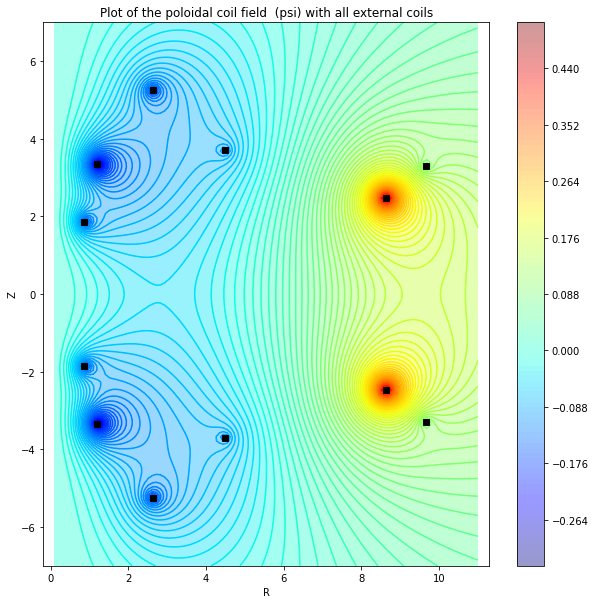
\includegraphics[height=0.75\textheight]{pics/coil_field.png}
   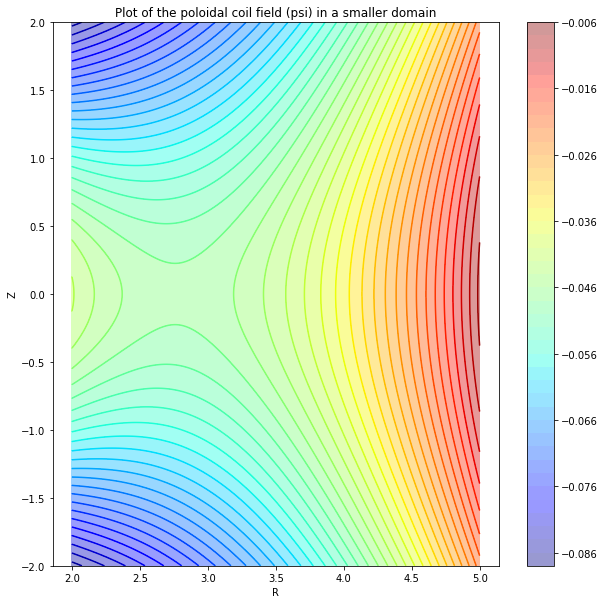
\includegraphics[height=0.75\textheight]{pics/coil_field_zoom.png}
   }\only<2-4>{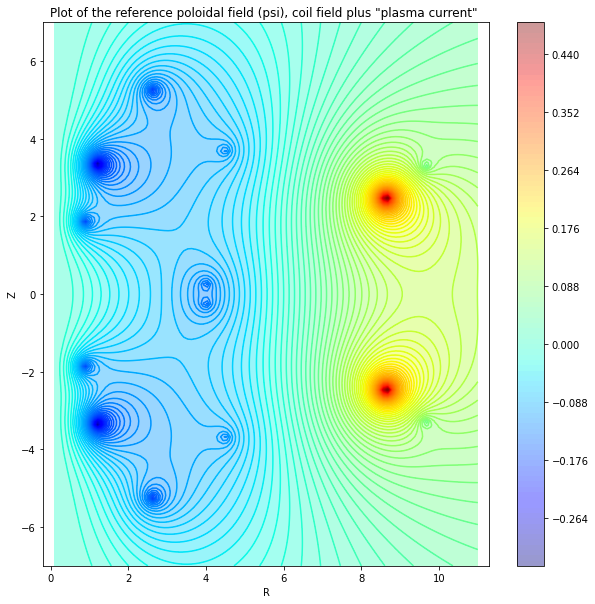
\includegraphics[height=0.75\textheight]{pics/full_field.png}
   }\only<2>{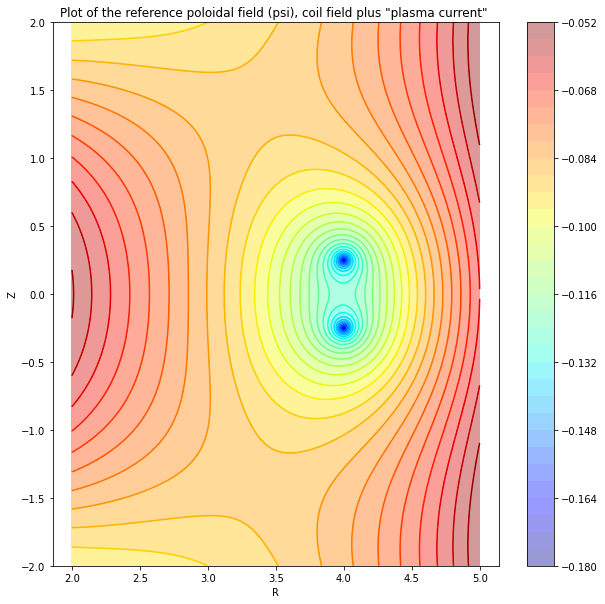
\includegraphics[height=0.75\textheight]{pics/full_field_zoom.png}
   }\only<3>{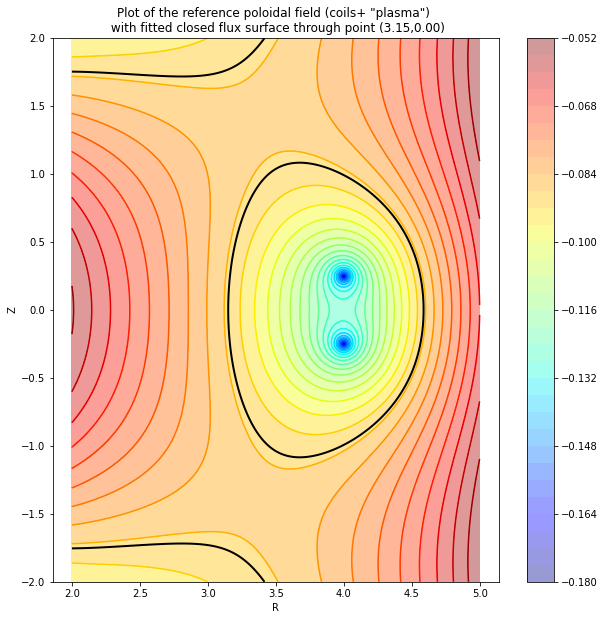
\includegraphics[height=0.75\textheight]{pics/full_field_zoom_contour.png}
   }\only<4>{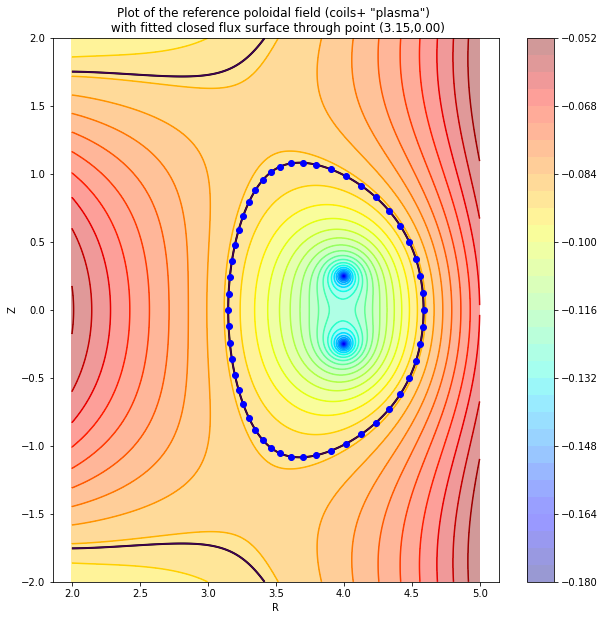
\includegraphics[height=0.75\textheight]{pics/full_field_zoom_curve_fit.png}
   }\\
  \begin{itemize}
   \only<1>{\item Symmetric coil field evaluated from a set of point sources}
   \only<2-4>{\item Add two 'plasma' current sources to generate a 'plasma' region: full field $=B_\text{ref}$}
   \item<3-4> Choose a closed flux surface \textc{$\Leftrightarrow$  'plasma'-vacuum boundary} \only<4>{\textc{$\Rightarrow$ fit parametrized curve!}}
  \end{itemize}

\end{frame}

\begin{frame}
 \frametitle{Fit parametrized curve to a contour}
 \centering\small
 \only<1>{
 \vspace{-2ex}
      \begin{columns}[t]
      \begin{column}{0.6\textwidth}
      \begin{itemize}
  \item Find periodic curve $R_c(t),Z_c(t)$ with a 'meaningful' parametrization (for example 'equal arc length')
  \item Fourier representation of $R_c,Z_c$ (up-down symmetry)
  \item Least squares minimization of the 'squared distance'  in the magnetic flux, sampled on a set of point along the curve:\\[1ex]\centerline{$
\min\left(\frac{1}{2}\sum_i \frac{|\Psi(R_c(t_i),Z_c(t_i))-\Psi_\text{contour}|^2}{|\Psi_\text{contour}|^2}+\frac{|B\cdot n_i|^2}{|B|^2}\right)$}
  \item Iteratively fit + increase mode number $m_\text{max}=4 \dots  12$
  \item[$\Rightarrow$] Accuracy seems limited to single precision (due to square...?) 
   \item But gives a good parametrization. \\
       Since BEAST needs only points, add a 2nd step:\\
   find the root to the contour in normal direction: \\[1ex] \centerline{ $\Psi\left((R_i+\alpha N_R),(Z_i+\alpha N_Z)\right) -\Psi_\text{contour}=0$} 
 \end{itemize}
      \end{column}
    \begin{column}{0.4\textwidth}
    \vspace{-4ex}\\
    \centering
    \hspace*{-3ex}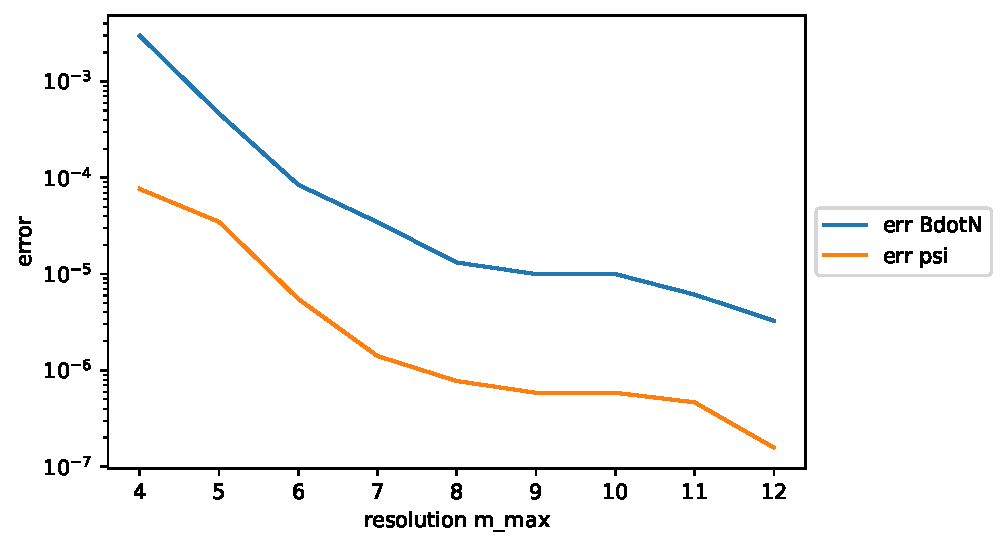
\includegraphics[width=1.2\textwidth]{pics/error_curve_fit.pdf}\\[-1ex]
       \textit{\scriptsize Error of the fitted curves with LS}\\[1ex]
         \hspace*{-3ex}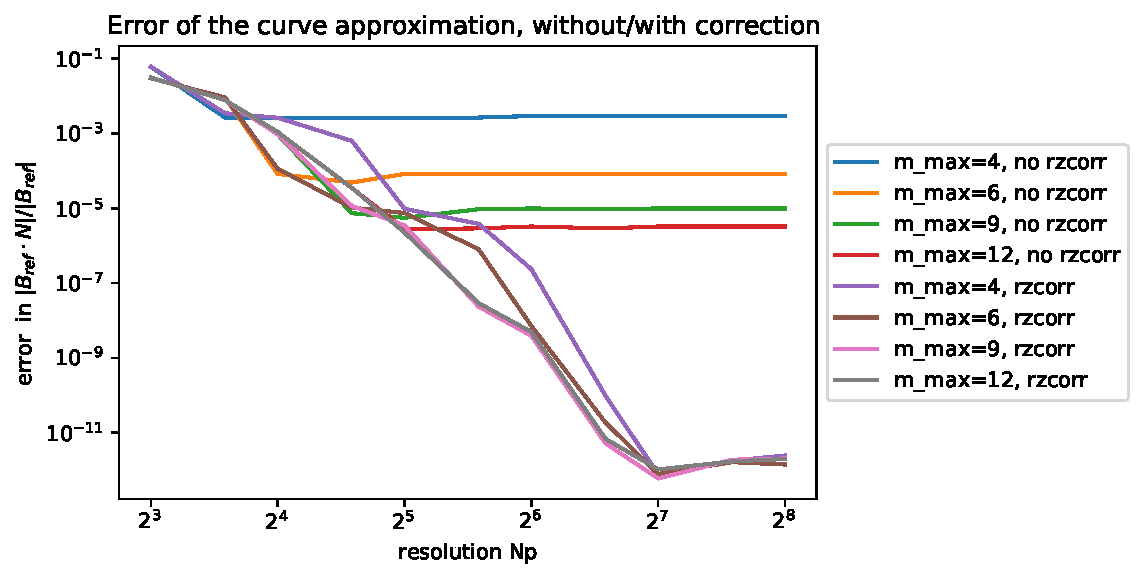
\includegraphics[width=1.2\textwidth]{pics/error_curve_approx.pdf}\\[-1ex]
       \textit{\scriptsize Approximation error of the normal $|B_\text{ref}\cdot N|/|B_\text{ref}|$  w/o and with correction}\\
    \end{column}
  \end{columns}
  }
  \only<2>{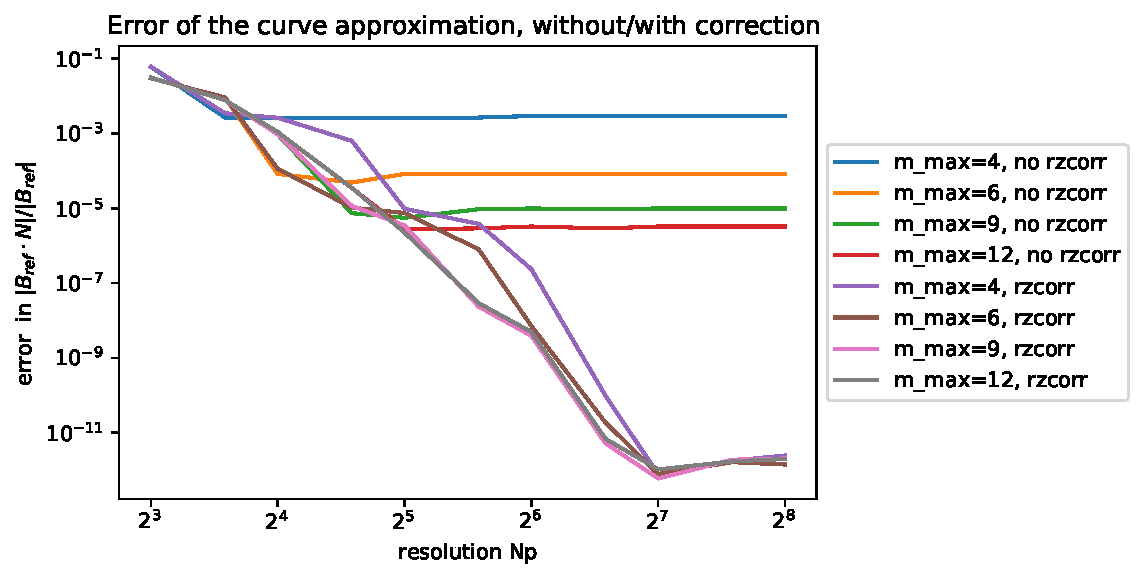
\includegraphics[height=0.72\textheight]{pics/error_curve_approx.pdf}\\[-1ex]
  $N_p$ is the number of points on the curve, $N$, $B_{ref}$ is the reference first at these points and $B_\text{ref}\cdot N$ is computed within BIEST. Machine precision reached at $N_p=128$\\
  \textc{$\Rightarrow$ Keep in mind: when comparing the field to $B_\text{ref}$, \\ we already have an approximation error of the normal direction $N$!}
  }
\end{frame}

\begin{frame}
 \frametitle{Testing the influence of the choice of $B_0$}
 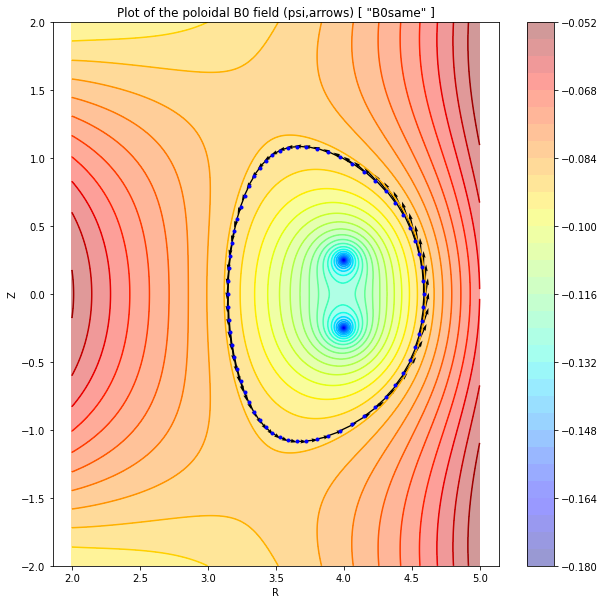
\includegraphics[width=0.24\textwidth]{pics/B0_same.png}
 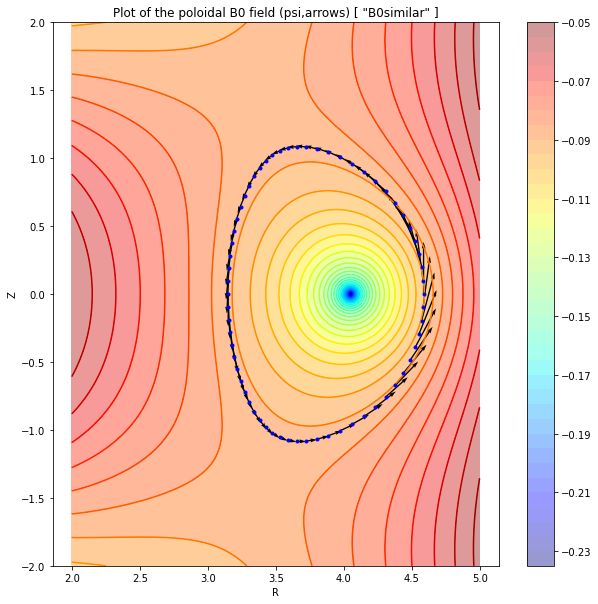
\includegraphics[width=0.24\textwidth]{pics/B0_similar.png}
 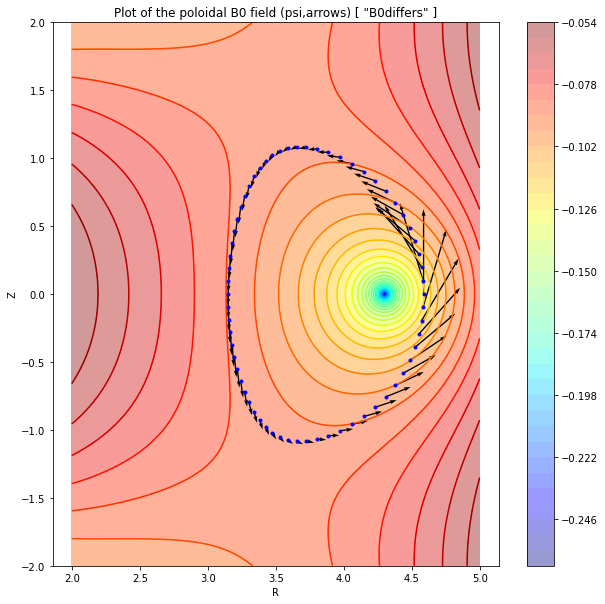
\includegraphics[width=0.24\textwidth]{pics/B0_differs.png}
 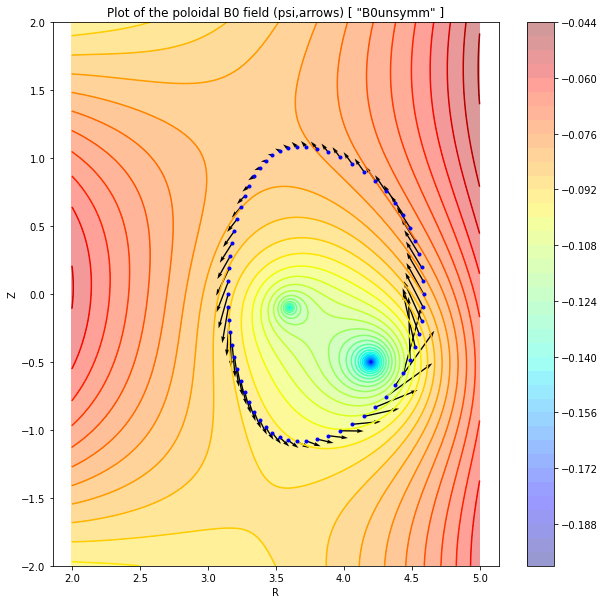
\includegraphics[width=0.24\textwidth]{pics/B0_unsymm.png}\\
 We will look at 4 cases, all have the same 'plasma' current: 
 \begin{enumerate}
  \item 'same': Set $B_0=B_\text{ref}$ (so that $\nabla \Phi=0$)
  \item 'similar': Change 'plasma' current soure position slightly $B_0\neq B_\text{ref}$
  \item 'differs': Change positions more
  \item 'unsymm.': Change positions more and make $B_0$ unsymmetric
 \end{enumerate}

\end{frame}

\begin{frame}
 \frametitle{Results: Case $B_0$ same as $B_\text{ref}$}
 \centering\small
 \begin{columns}[t]
  \begin{column}{0.38\textwidth}
   \hspace*{-0.8cm}\only<1>{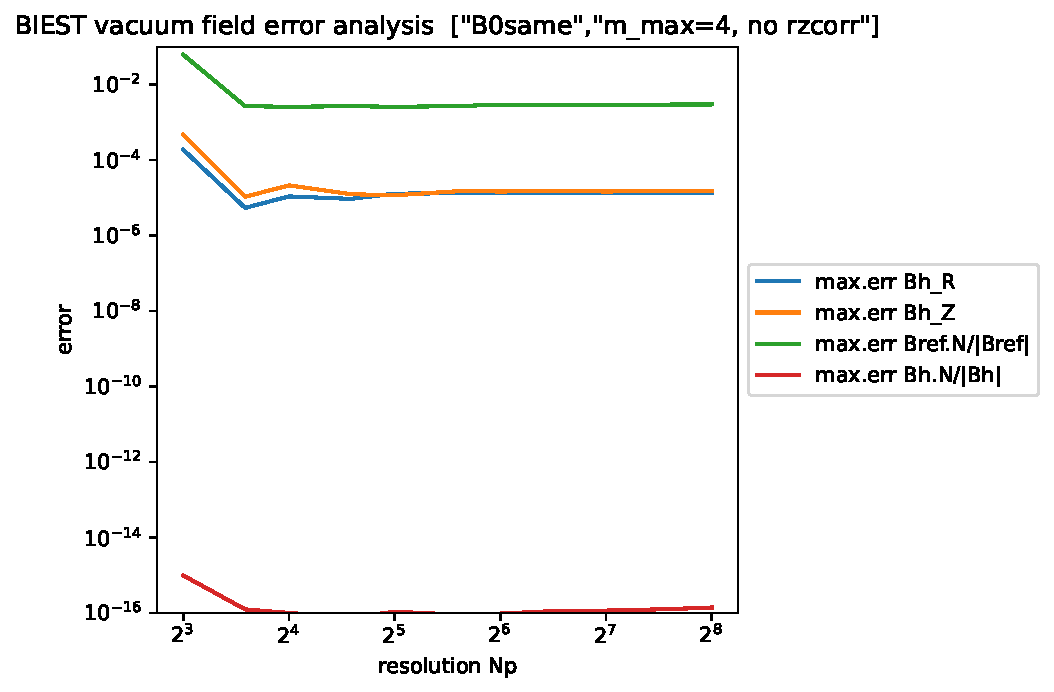
\includegraphics[height=0.7\textheight,trim=0 0 150 0,clip]{pics/BIEST_vf_err_B0same_m_max=4_norzcorr.pdf}
   }\only<2>{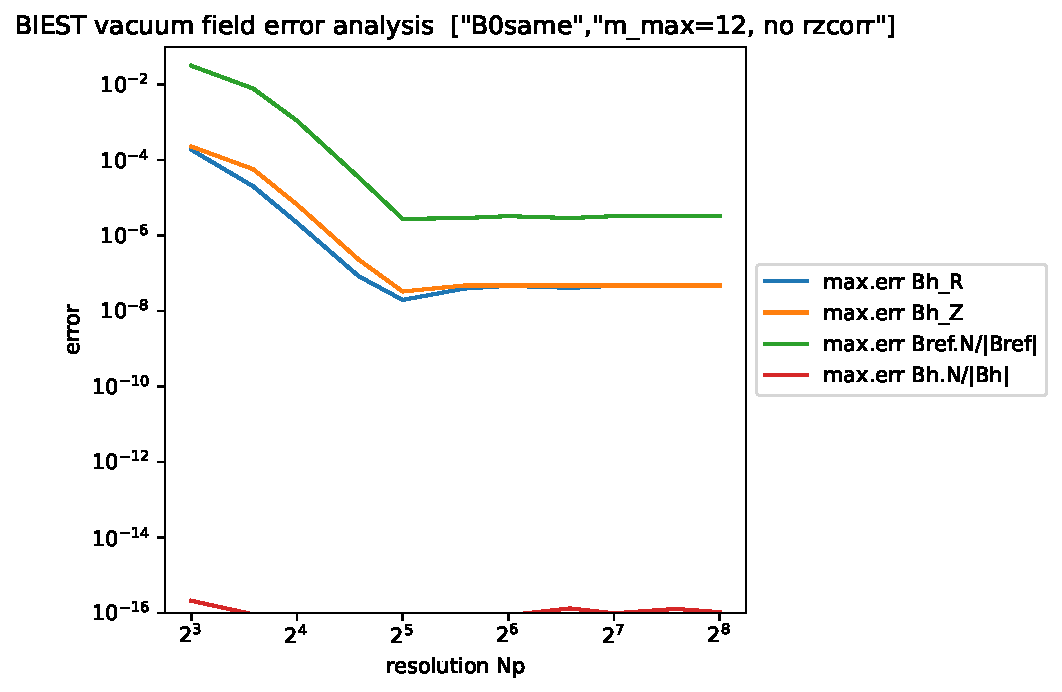
\includegraphics[height=0.7\textheight,trim=0 0 150 0,clip]{pics/BIEST_vf_err_B0same_m_max=12_norzcorr.pdf}}
  \end{column}
 \begin{column}{0.6\textwidth}
   \only<1>{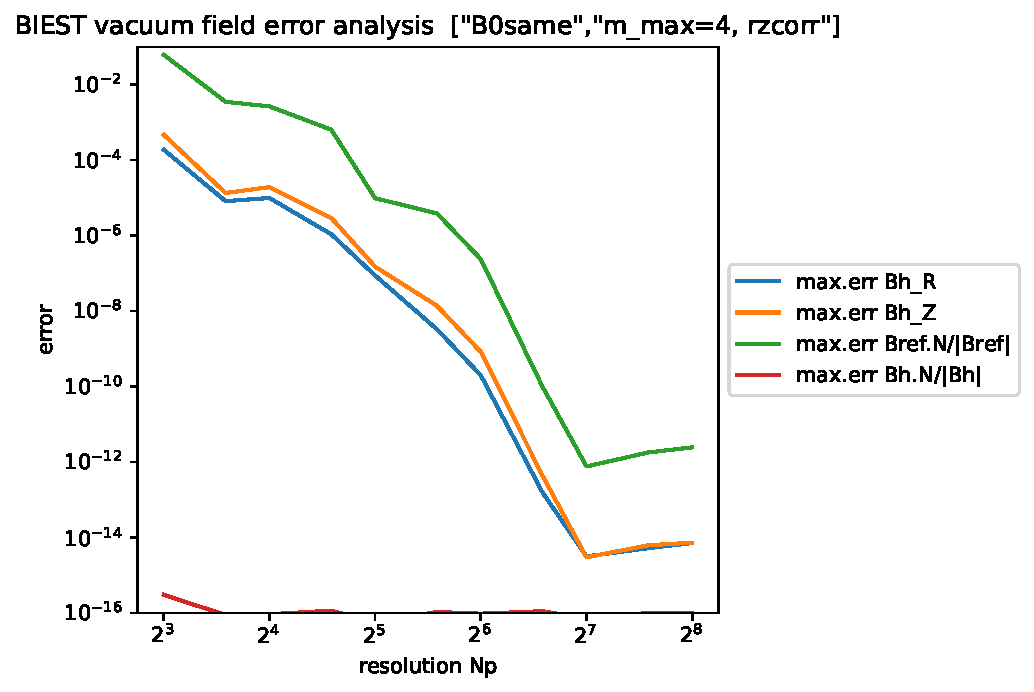
\includegraphics[height=0.7\textheight]{pics/BIEST_vf_err_B0same_m_max=4_rzcorr.pdf}
   }\only<2>{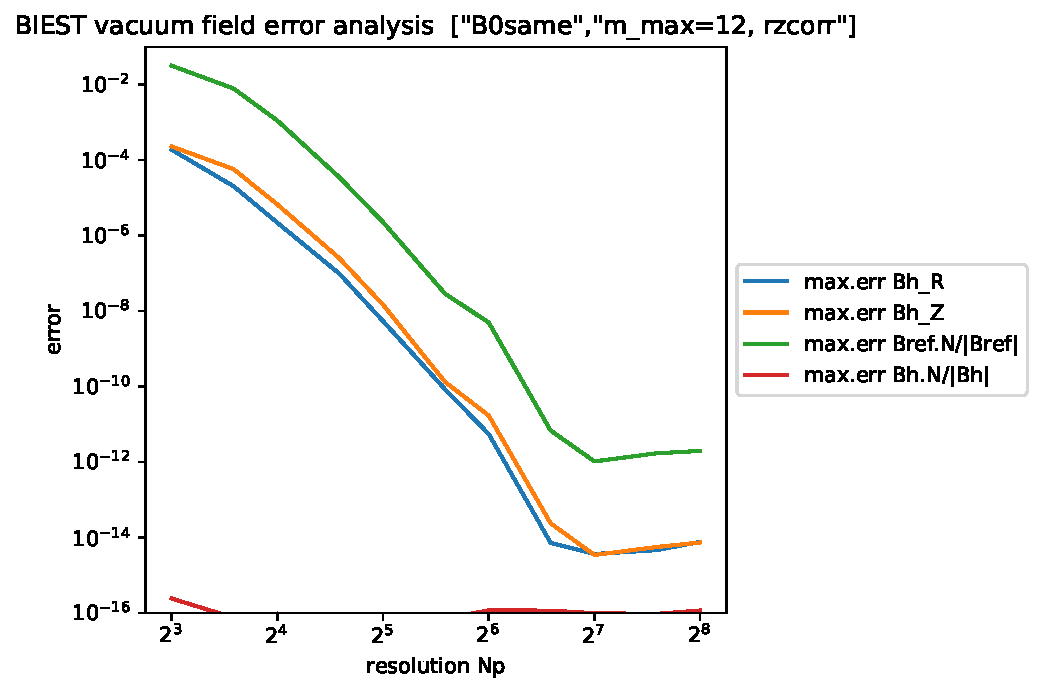
\includegraphics[height=0.7\textheight]{pics/BIEST_vf_err_B0same_m_max=12_rzcorr.pdf}}
  \end{column}
 \end{columns}\vspace{-2ex}
  w/o and with correction of the curve, \only<1>{$m_\text{max}=4$}\only<2>{$m_\text{max}=12$. $B\cdot N=0$ satisfied point-wise.}\\
  \textc{$\Rightarrow$ error of magnetic field lower than the curve approximation error}\\
 \only<1>{\textc{$\Rightarrow$ error without correction dominated by curve appoximation}}
 \only<2>{\textc{$\Rightarrow$ error without correction dominated by curve appoximation, but same up to $N_p=32$}}

\end{frame}


\begin{frame}
 \frametitle{Results: Case $B_0$ similar}
 \centering\small
 \begin{columns}[t]
  \begin{column}{0.38\textwidth}
   \hspace*{-0.8cm}\only<1>{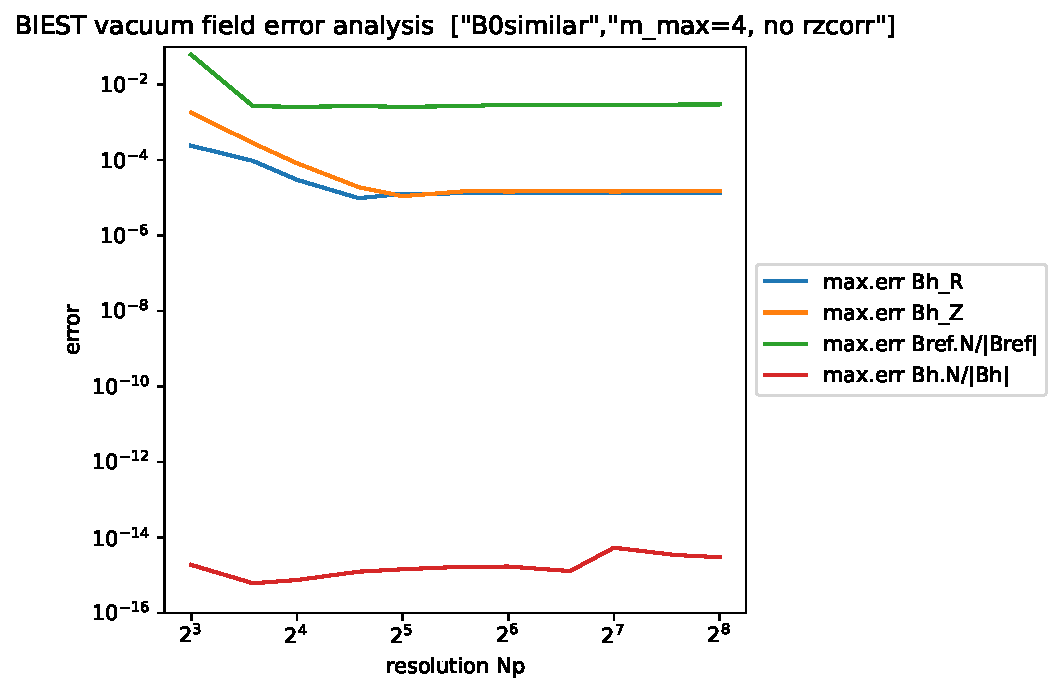
\includegraphics[height=0.7\textheight,trim=0 0 150 0,clip]{pics/BIEST_vf_err_B0similar_m_max=4_norzcorr.pdf}
   }\only<2>{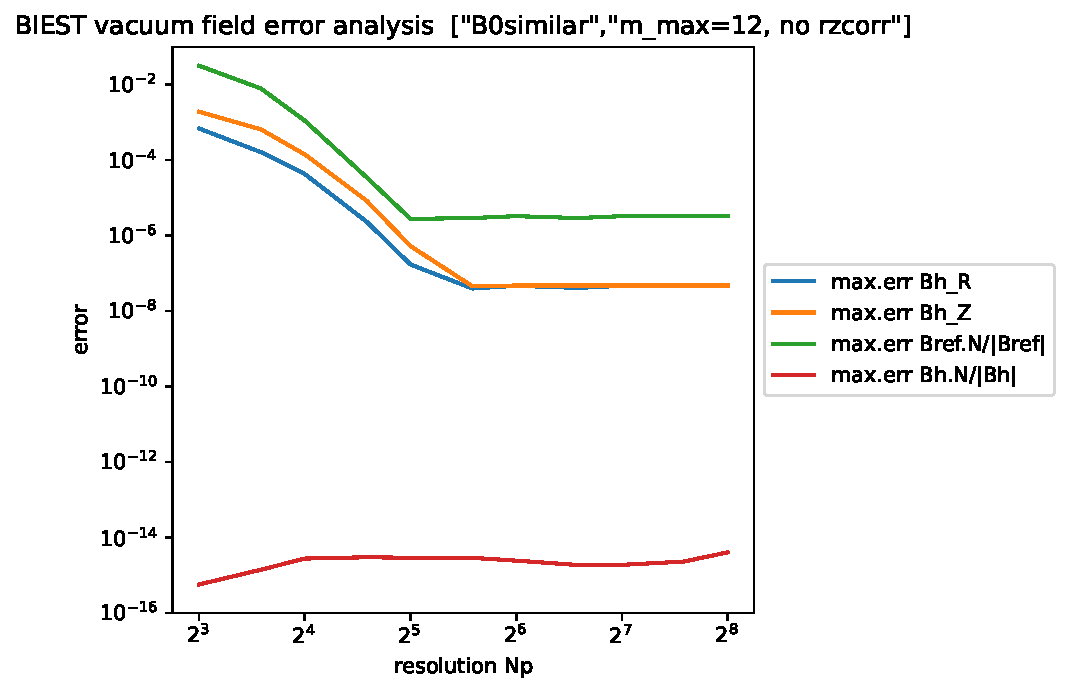
\includegraphics[height=0.7\textheight,trim=0 0 150 0,clip]{pics/BIEST_vf_err_B0similar_m_max=12_norzcorr.pdf}}
  \end{column}
 \begin{column}{0.6\textwidth}
   \only<1>{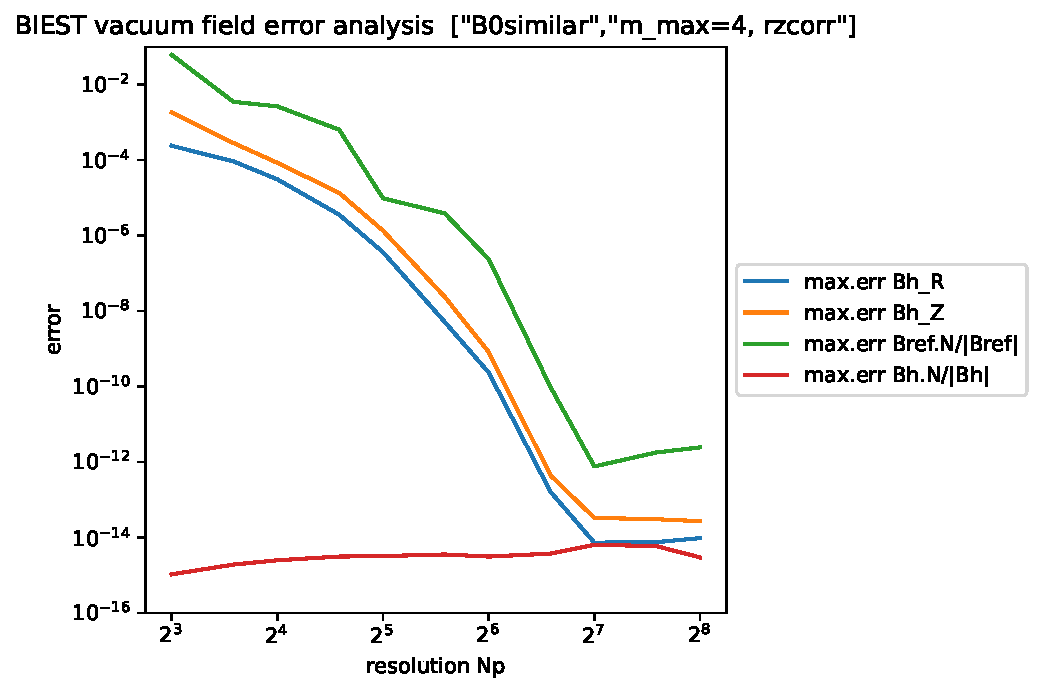
\includegraphics[height=0.7\textheight]{pics/BIEST_vf_err_B0similar_m_max=4_rzcorr.pdf}
   }\only<2>{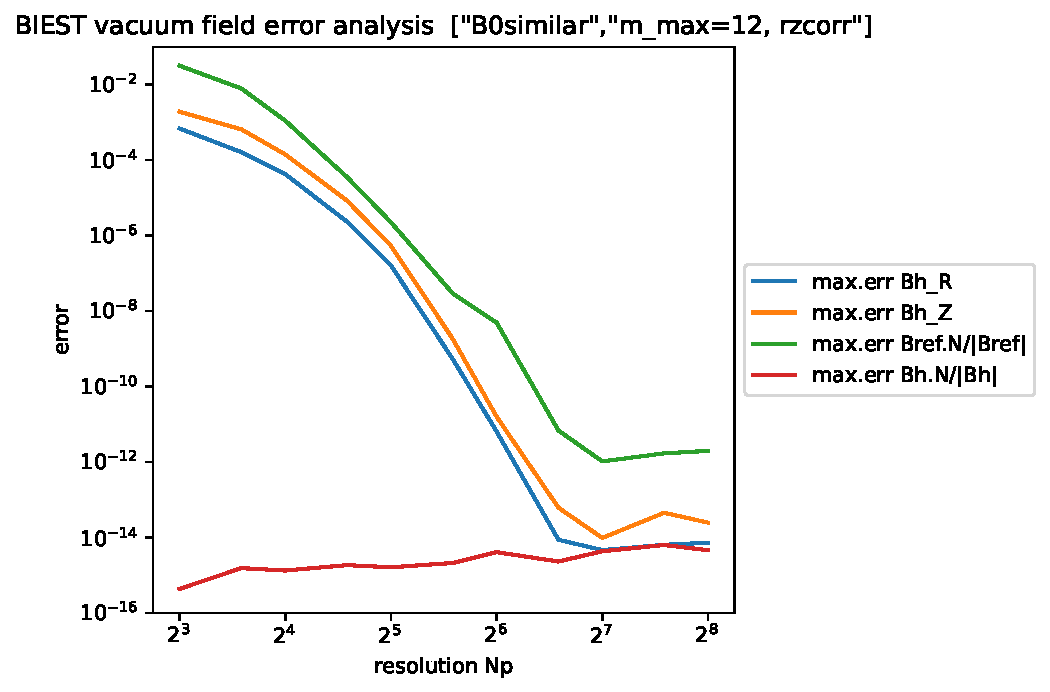
\includegraphics[height=0.7\textheight]{pics/BIEST_vf_err_B0similar_m_max=12_rzcorr.pdf}}
  \end{column}
 \end{columns}\vspace{-2ex}
 w/o and with correction of the curve, \only<1>{$m_\text{max}=4$}\only<2>{$m_\text{max}=12$. $B\cdot N=0$ satisfied point-wise.}\\
  \textc{$\Rightarrow$ error of magnetic field smaller than the curve approximation error}\\
 \only<1>{\textc{$\Rightarrow$ error without correction dominated by curve appoximation}}
 \only<2>{\textc{$\Rightarrow$ error without correction dominated by curve appoximation, but same up to $N_p=32$}}

\end{frame}

\begin{frame}
 \frametitle{Results: Case $B_0$ differs}
 \centering\small
 \begin{columns}[t]
  \begin{column}{0.38\textwidth}
   \hspace*{-0.8cm}{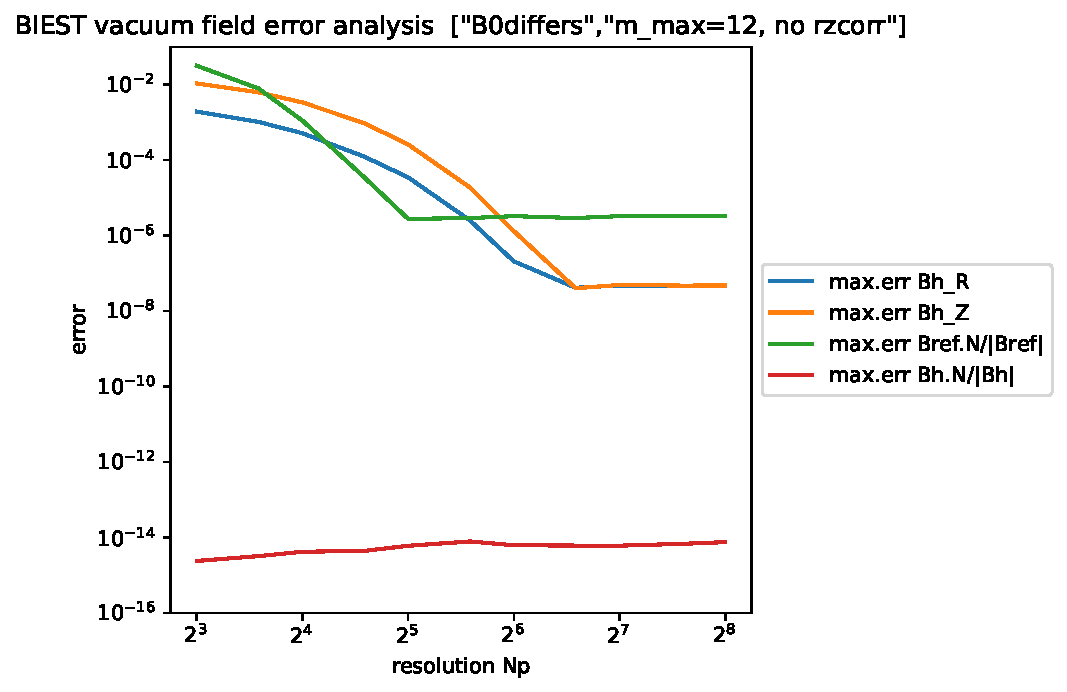
\includegraphics[height=0.7\textheight,trim=0 0 150 0,clip]{pics/BIEST_vf_err_B0differs_m_max=12_norzcorr.pdf}}
  \end{column}\vspace{-2ex}
 \begin{column}{0.6\textwidth}
   {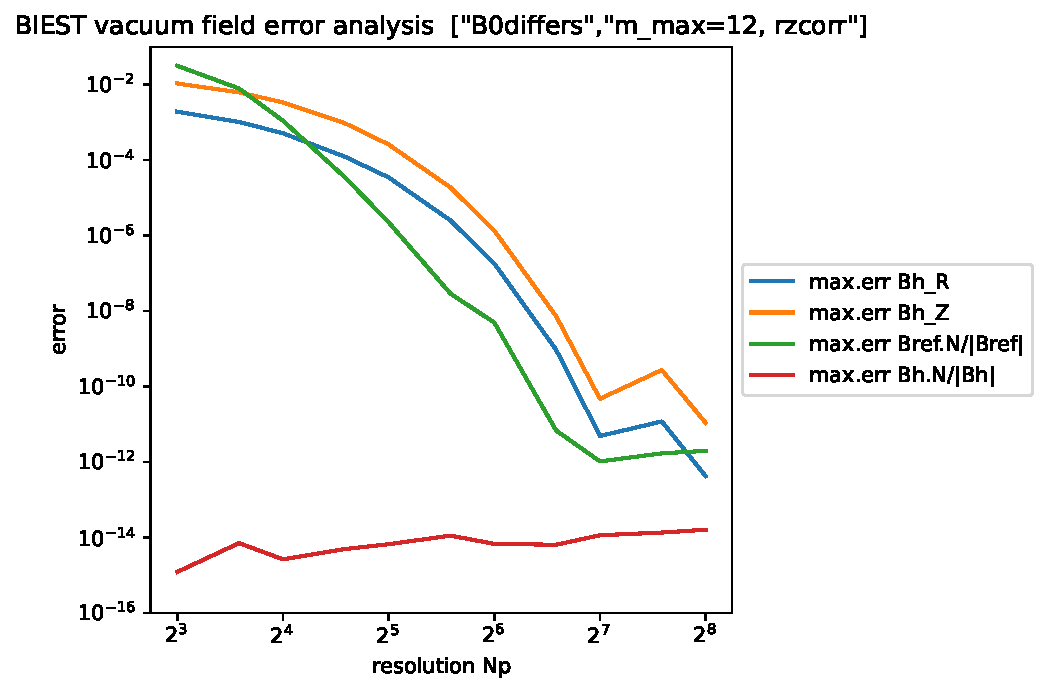
\includegraphics[height=0.7\textheight]{pics/BIEST_vf_err_B0differs_m_max=12_rzcorr.pdf}}
  \end{column}
 \end{columns}
 w/o and with correction of the curve, {$m_\text{max}=12$}. $B\cdot N=0$ satisfied point-wise.\\
  \textc{$\Rightarrow$ error of magnetic field now larger than the curve approximation error}\\
 {\textc{$\Rightarrow$ error without correction dominated by curve appoximation, but same up to $N_p=64$}}

\end{frame}

\begin{frame}
 \frametitle{Results: Case $B_0$ unsymmetric}
 \centering\small
 \begin{columns}[t]
  \begin{column}{0.38\textwidth}
   \hspace*{-0.8cm}{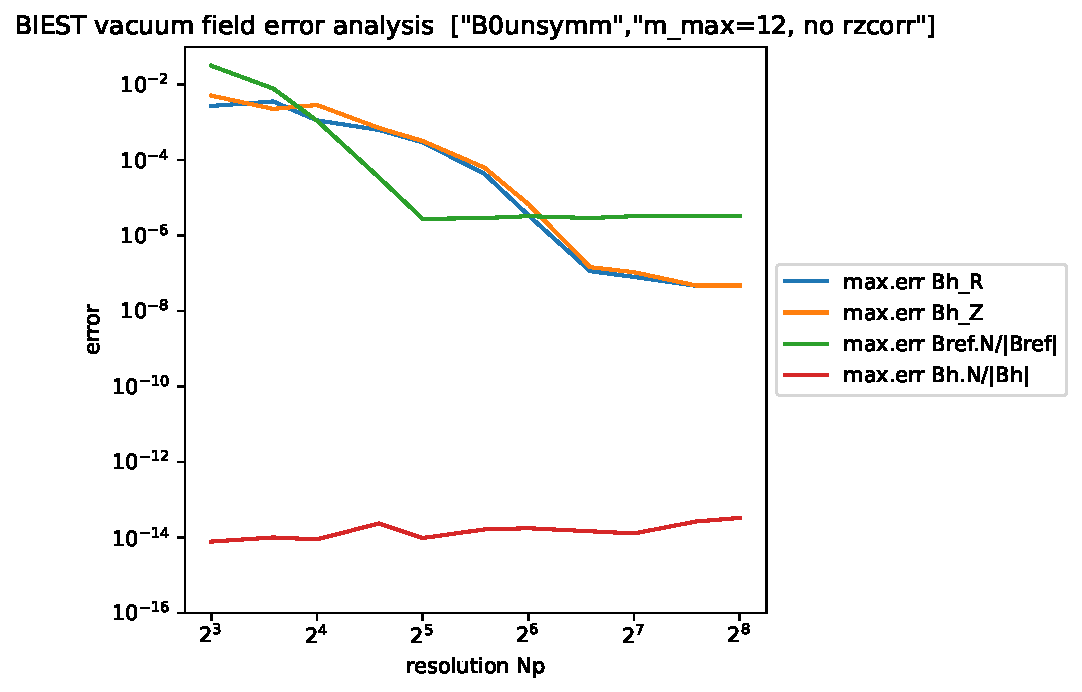
\includegraphics[height=0.7\textheight,trim=0 0 150 0,clip]{pics/BIEST_vf_err_B0unsymm_m_max=12_norzcorr.pdf}}
  \end{column}
 \begin{column}{0.6\textwidth}
   {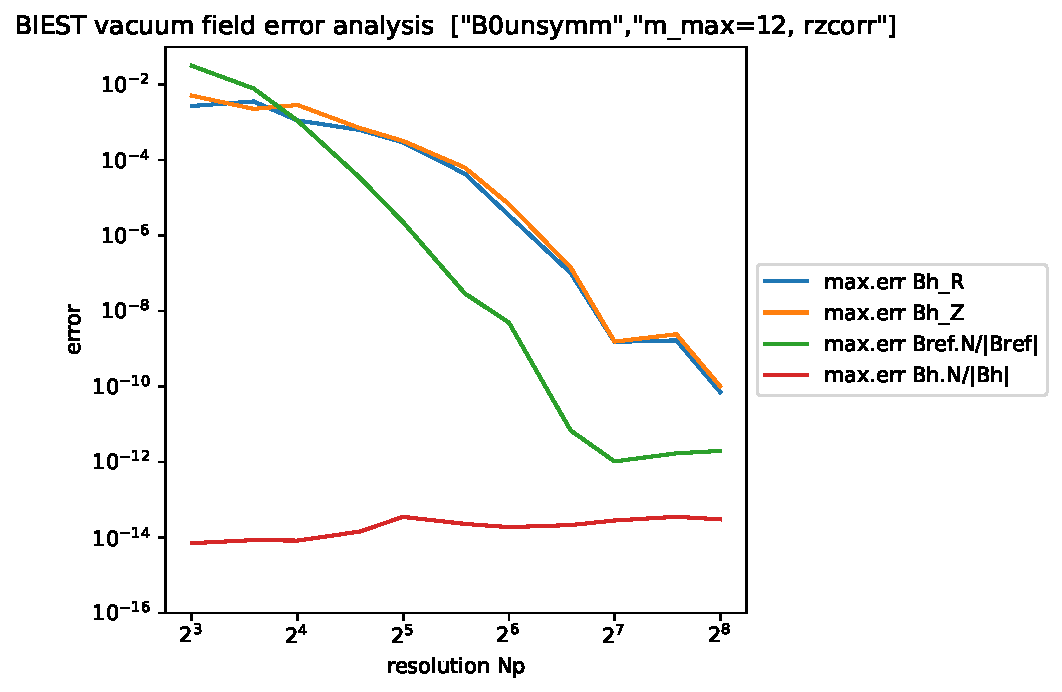
\includegraphics[height=0.7\textheight]{pics/BIEST_vf_err_B0unsymm_m_max=12_rzcorr.pdf}}
  \end{column}
 \end{columns}
 w/o and with correction of the curve, {$m_\text{max}=12$}\\
  \textc{$\Rightarrow$ error of magnetic field now larger than the curve approximation error}\\
 {\textc{$\Rightarrow$ error without correction dominated by curve appoximation, but same up to $N_p=48$}}

\end{frame}

\begin{frame}
 \frametitle{Conclusion on the results}
 \begin{itemize}
  \item The choice of the 'plasma' current position for $B_0$ has a strong influence on the accuracy of the result
  \item Error in the fields behaves similar to the error of the geometry approximation
  \item convergence behavior is spectral but also affected for the worst case
 \end{itemize}

\end{frame}


\begin{frame}
  \frametitle{BIEST compilation, python interface} 
  \small
\begin{itemize}
  \item Using \texttt{Makefile} means that changes in compilers/libraries must be edited locally, without being able to save the configuration in the repo...
  \item Managed to compile on my machine (linux, ubuntu) with 
        \texttt{gcc, blas, lapack, fftw3} 
        after installing all these libraries on my machine, and uncommenting the correct lines in the Makefile, it worked.
  \item  Managed to compile on cluster (linux, module env. for libraries) with           \texttt{gcc, mkl, fftw3}  \\
         added path to the loaded libraries to the Makefile (\texttt{-L} and \texttt{-I} flags) and executable needs module path in \texttt{LD\_LIBRARY\_PATH}, seems cluster specific)\\
         compilation with INTEL 21.4 failed first, fixed with loading new version of gcc as well!
   \item Forked Bharats \texttt{virtual\_casing}\footnote{\tiny\url{github.com/hiddenSymmetries/virtual-casing}} repo, as a blueprint, to my github as \texttt{BIEST\_to\_python}\footnote{\tiny\url{github.com/fhindenlang/biest_to_python}}
   \item Setup only for the \textc{\texttt{vacuum\_field} application}, by modifying the cpp file for the \texttt{pybind11} tool. With \texttt{cmake} and \texttt{pybind11} a shared object is built that can be called from python (!) 
   \item[$\Rightarrow$] \textc{Can call \texttt{setup,computeBdotN,computeGradPhi} from python (3D-arrays ordered correctly \& flattened), simply by placing the generated \texttt{.so} file into the folder of the python script.}
\end{itemize}
   
\end{frame}


\begin{frame}
  \frametitle{Code specific questions} 
  \small
   
\begin{itemize}
  \item The main C++ code of \texttt{BIEST} is written with only templates, and thus they are only included in the compilation against a \texttt{.cpp} file, being an executable (or an interface?). What is the reason this is done like this? \\
  \textit{\tiny Answer: easier to compile against other codes, since no need to compile Biest as a library first.}
  \item How do you choose the coordinate system? (right now its $(R,\phi,Z)$, which is then also used for the vector components)\\
  \textit{\tiny Answer: $(R,\phi,Z)$ is actually cartesian $(x,y,z)$, but can be used likewise in the axi-symmetric case...}
  \item How do you then control axi-symmetry, only by choosing one 'toroidal' integration point?\\
  \textit{\tiny Answer: Yes, if only one plane is given, its supposed to be axi-sym. If more planes are given, coordinates must then be cartesian $(x,y,z)$!!}
  \item Is there a reason for setting \texttt{NFP=4} in the axi-symmetric case?\\
  \textit{\tiny Answer: Yes, its again a trick for the axi-symmetric case to get enough integration points!}
  \item Can one input the geometry with a certain set of points and get the result on a different/higher sampled set of points? (useful for GVEC and also for error analysis)\\
  \textit{\tiny Answer: Yes, its the last Nt,Np parameters in the setup}
   \item Can one evaluate the field(s) at other points in the outer domain, for post-processing?\\
   \textit{\tiny Answer: An additional routine will be added b Dhairya (thanks!)}
\end{itemize}
   
\end{frame}

\begin{frame}
 \frametitle{More physical questions}
 \begin{itemize}
  \item For the free-boundary computations (especially in 3D), we need to compute the coil field on the plasma boundary. \\ If we can define a smooth 'outer domain boundary' (excluding the coils, including the plasma domain): \\
  is it possible to use BIEST to evaluate the coil field once at that boundary and use it to evaluate the field on the plasma boundary?\\
    \textit{\scriptsize Answer: Possible via virtual casing, but not recommendable from an accuracy vs. computational effort view. Should be computed via Biot-Savard directly from the coils (without Mgrid file!) }
  \item Instead of computing an additional  contribution to $B_0$ representing the toroidal current from a loop around the plasma, could we just pass that current as a constraint? \\
    \textit{\scriptsize Answer: Dhairya will look into this, it should be possible to pass $B_{coil}$ and only the current from the loop integral}
\end{itemize}
\end{frame}


\begin{frame}
\frametitle{Appendix}
\end{frame}


\begin{frame}
 \frametitle{Results: Case $B_0$ unsymmetric: Increase $N_p$ of output}
 \centering\small
  \only<1>{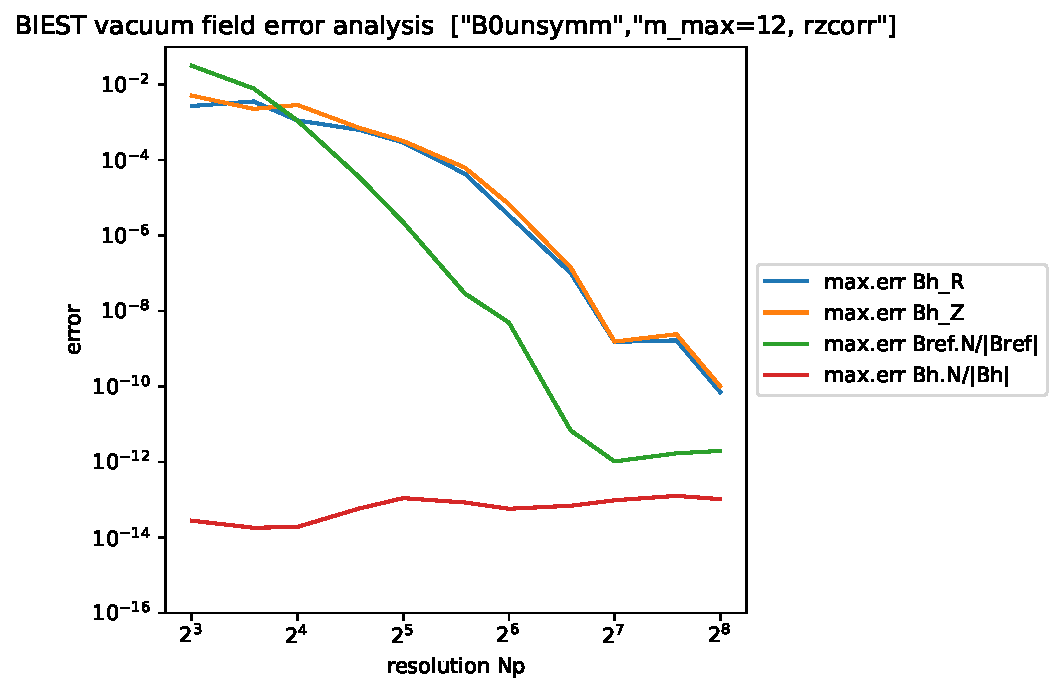
\includegraphics[height=0.7\textheight]{pics/BIEST_vf_err_B0unsymm_1Np_m_max=12_rzcorr.pdf}\\$N_p^\text{out}=N_p$
  }\only<2>{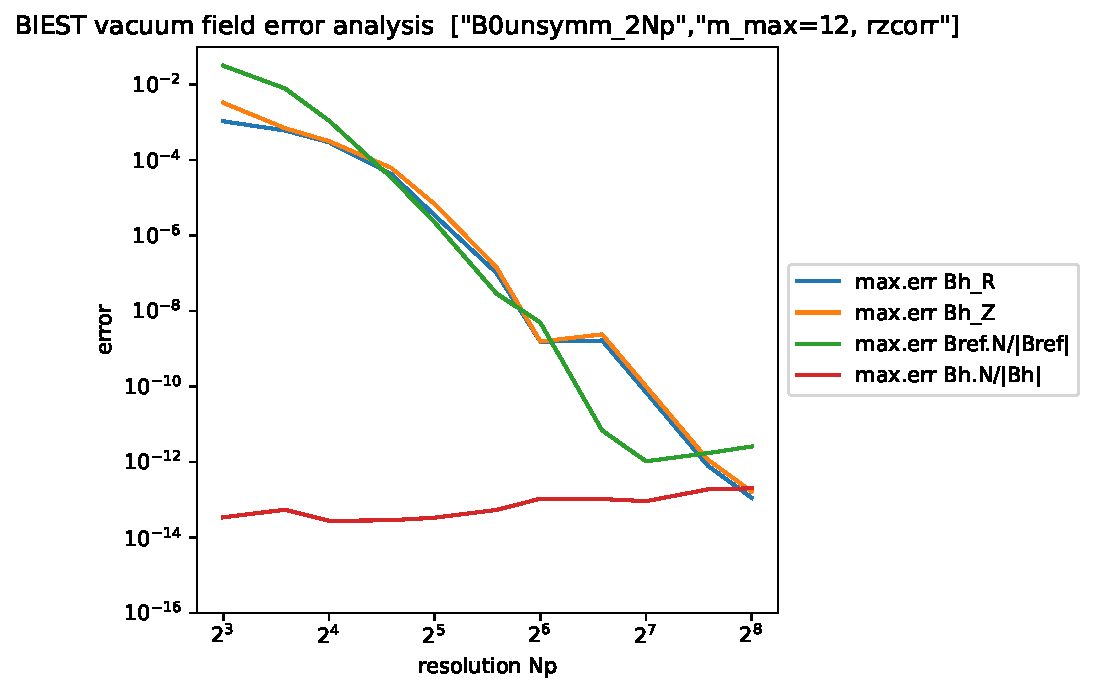
\includegraphics[height=0.7\textheight]{pics/BIEST_vf_err_B0unsymm_2Np_m_max=12_rzcorr.pdf}\\$N_p^\text{out}=2 N_p$
  }\only<3>{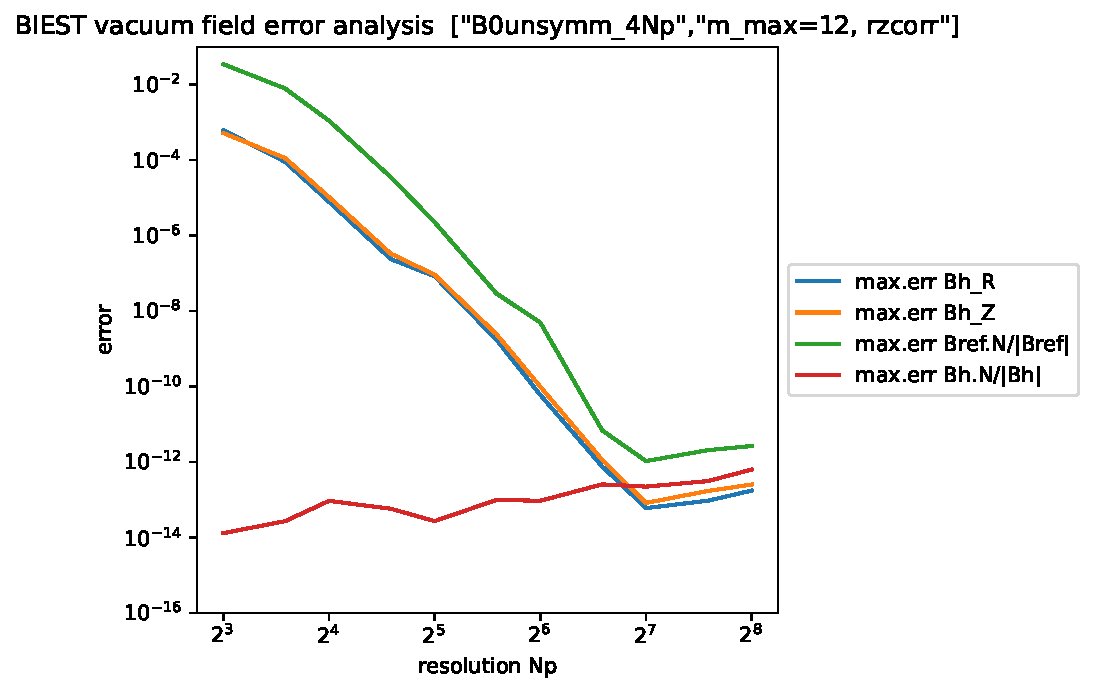
\includegraphics[height=0.7\textheight]{pics/BIEST_vf_err_B0unsymm_4Np_m_max=12_rzcorr.pdf}\\$N_p^\text{out}=4 N_p$
  }\\
  \textc{$\Rightarrow$ Increasing the number of output points increases the cost, and improves the error   ($B_0\cdot N$ is higher resolved)}\\
  \textc{$\Rightarrow$ Same errors for same $N_p^\text{out}$. Note that increasing $N_p$ is not exactly the same!}
 

\end{frame}

\begin{frame}
 \frametitle{Results: Case $B_0$ similar: Increase $N_p$ of output}
 \centering\small
  \only<1>{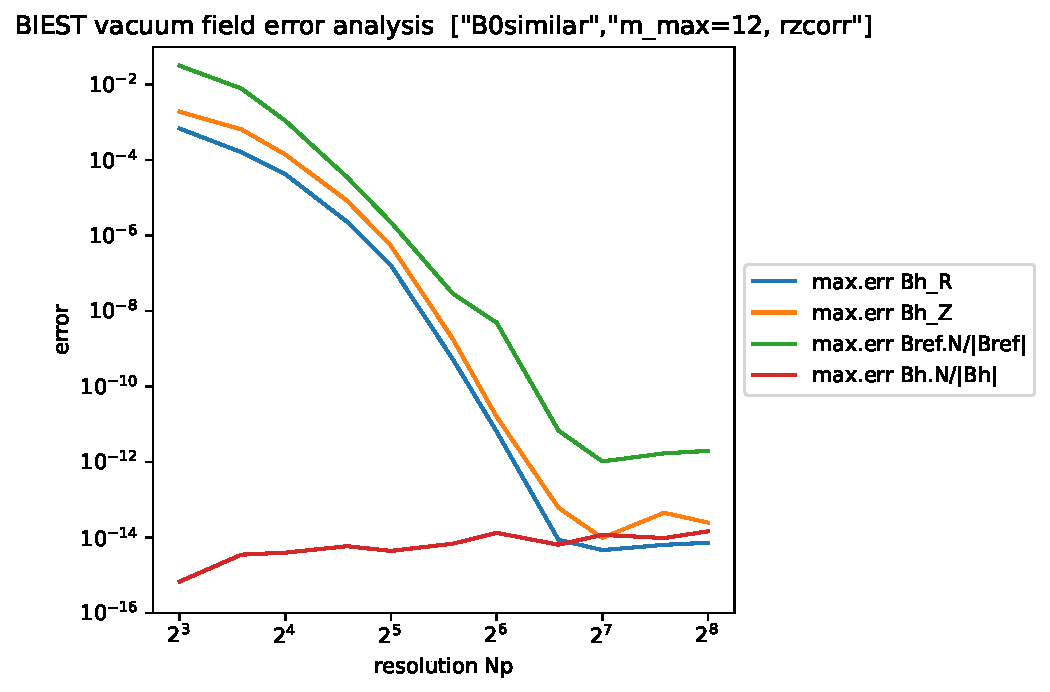
\includegraphics[height=0.7\textheight]{pics/BIEST_vf_err_B0similar_1Np_m_max=12_rzcorr.pdf}\\$N_p^\text{out}=N_p$
  }\only<2>{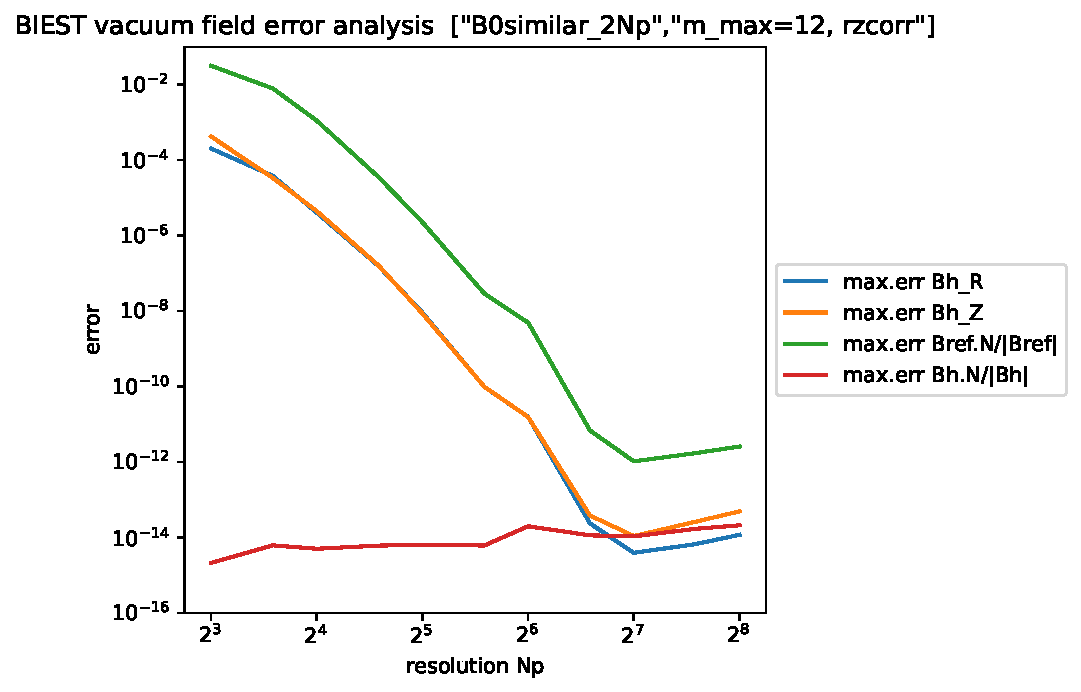
\includegraphics[height=0.7\textheight]{pics/BIEST_vf_err_B0similar_2Np_m_max=12_rzcorr.pdf}\\$N_p^\text{out}=2 N_p$
  }\only<3>{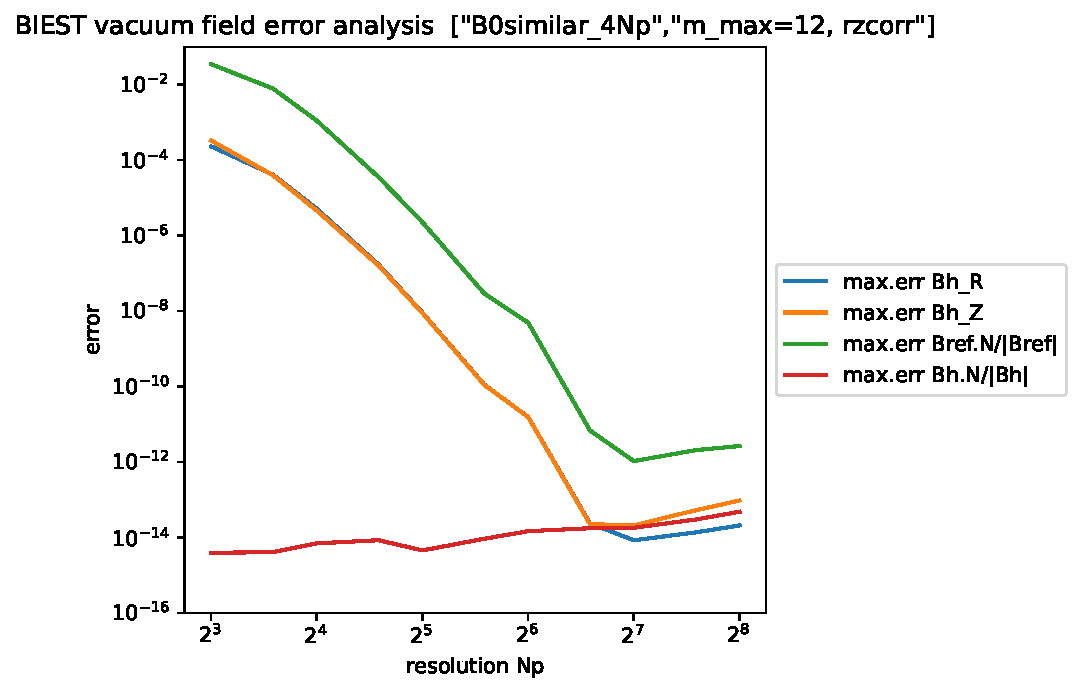
\includegraphics[height=0.7\textheight]{pics/BIEST_vf_err_B0similar_4Np_m_max=12_rzcorr.pdf}\\$N_p^\text{out}=4 N_p$
  }\\
  \textc{$\Rightarrow$ Increasing the number of output points increases the cost but error remains similar, thus here $B_0\cdot N$ is already well resolved}\\
 

\end{frame}

\begin{frame}
 \frametitle{2D Testcase with $B_\text{ref}$ unsymmetric}
 \small\centering
 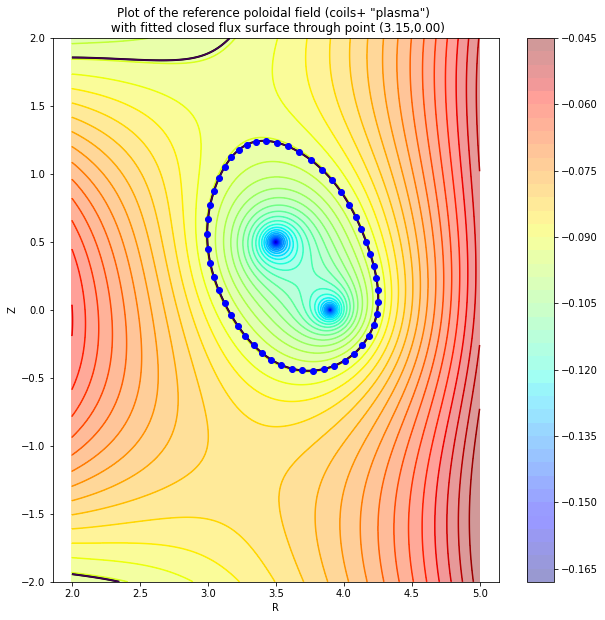
\includegraphics[height=0.75\textheight]{pics/Bref_unsymm_full_field_zoom_curve_fit.png}
   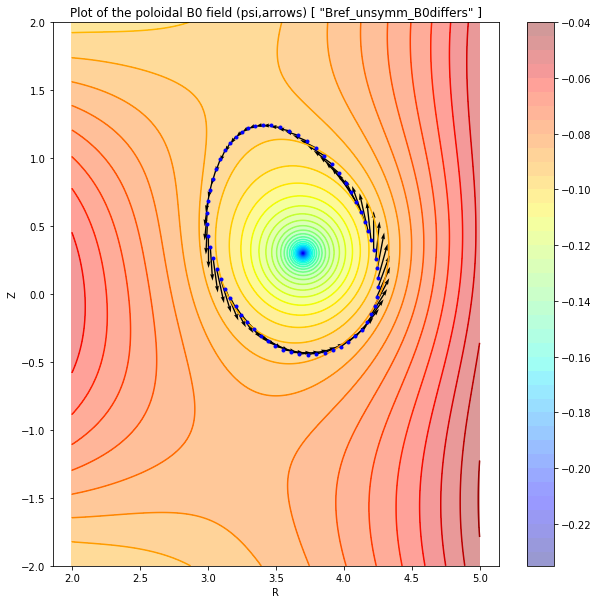
\includegraphics[height=0.75\textheight]{pics/Bref_unsymm_B0_differs.png}\\
  \begin{itemize}
   \item Fully unsymmetric flux surface (left)
   \item $B_0$  including a single 'plasma' current differs (right)
  \end{itemize}
 \end{frame}
 
\begin{frame}
 \frametitle{Results: $B_\text{ref}$ unsymmetric}
  \small\centering
 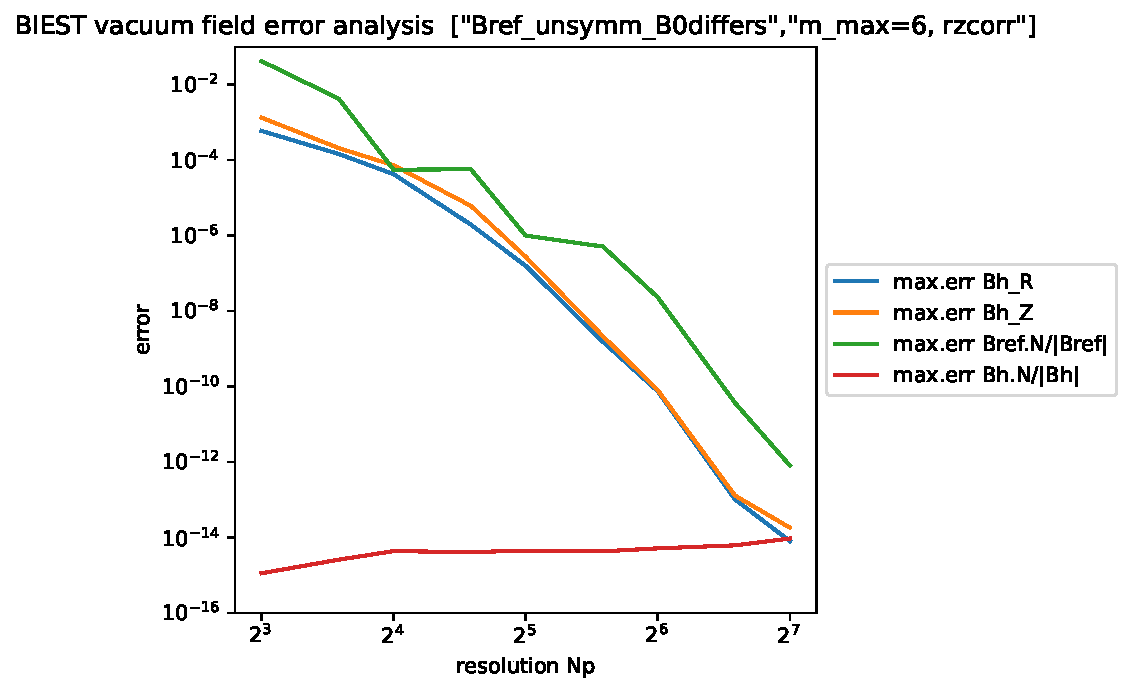
\includegraphics[height=0.7\textheight]{pics/BIEST_vf_err_Bref_unsymm_B0differs_m_max=6_rzcorr.pdf}\\$N_p^\text{out}=4 N_p$
  \\
  \textc{$\Rightarrow$ Axisymmetric case ($N_t=1,NFP=4$ behaves as expected. Same results for '3D' case with $N_t=4,NFP=1$.\\}
  
 
\end{frame}


\begin{frame}
 \frametitle{Results: $B_\text{ref}$ unsymmetric, 3D test! }
  \small\centering
  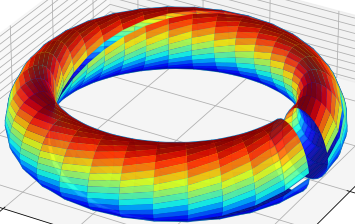
\includegraphics[height=0.4\textheight]{pics/Bref_unsymm_screw1_surf.png}\hspace*{-1cm}
 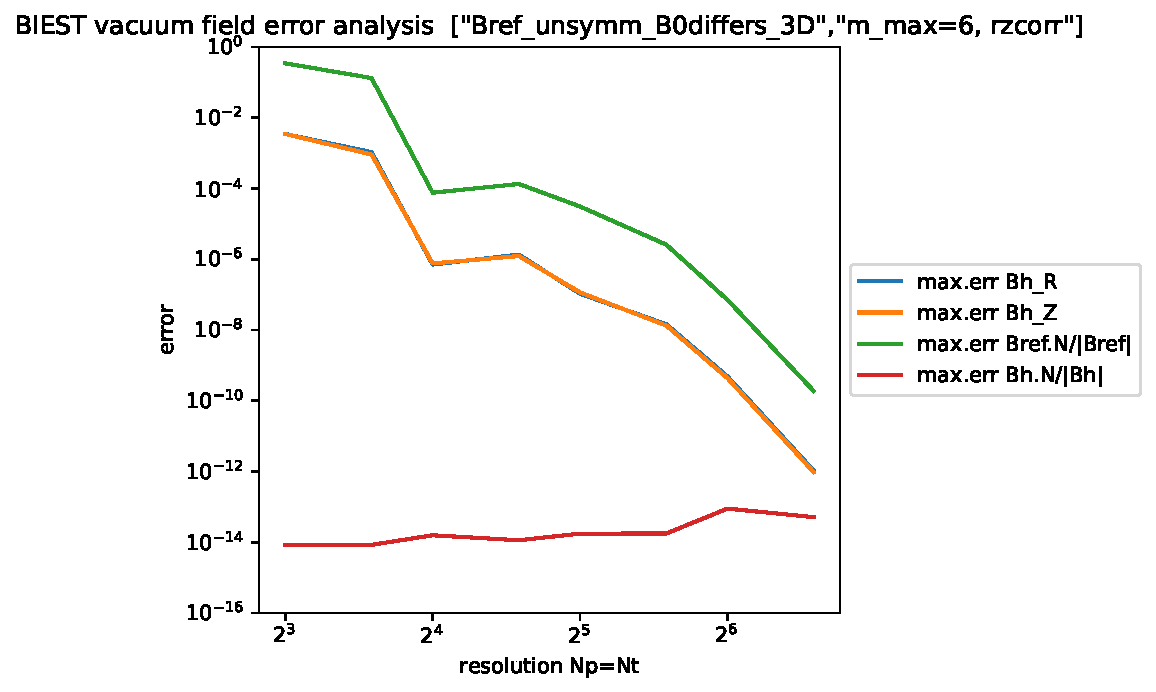
\includegraphics[height=0.7\textheight]{pics/BIEST_vf_err_Bref_unsymm_B0differs_3Dscrew1_m_max=6_rzcorr.pdf}\\$N_p^\text{out}=4 N_p$ , \textc{$N_t=N_p$}
  \\
  \textc{Full 3D} testcase from the axi-symmetric testcase by adding a 'Moebius torque' $R(\thet,\phi)=r(\theta + \phi)$ \\
  \textc{$\Rightarrow$ Converges, but slightly slower, } (max. resolution: $96x96$ input $4x96x4x96$ output!)
\end{frame}
% 

% \begin{frame}
%   \frametitle{ B and J fields} 
%   \small\centering
%    \only<1>{ \includegraphics[width=0.9\textwidth]{pics/w7a_axisym_r21_vmecinit_B_J_mag.png}\\$|B|,|J|$\\
%   }\only<2>{ \includegraphics[width=0.9\textwidth]{pics/w7a_axisym_r21_vmecinit_Bx_Jx.png}\\$B_R,J_R$ \\
%   }\only<3>{ \includegraphics[width=0.9\textwidth]{pics/w7a_axisym_r21_vmecinit_By_Jy.png}\\$B_{tor},J_{tor}$
%   }\only<4>{ \includegraphics[width=0.9\textwidth]{pics/w7a_axisym_r21_vmecinit_Bz_Jz.png}\\$B_Z,J_Z$
%   }
%   \begin{itemize}
%    \item Magnitude of $2.2<|B|<2.5$ and  $2.3e2<|J|< 1.5e6$  \\ (SI units, $J=\frac{1}{\mu_0}\nabla\times B$)
%    \item $J$ is smooth
%  \end{itemize} 
% \end{frame}
% %\subsection{Comparison of VMEC and GVEC solutions}
% 
% 
% 
% \begin{frame}
%   \frametitle{Force balance error of VMEC, init(A)} 
%   \small\centering
%    \only<1>{ \includegraphics[width=0.9\textwidth]{pics/w7a_axisym_r21_vmecinit_iter0000000.png}\\iter=0\\
%   }\only<2>{ \includegraphics[width=0.9\textwidth]{pics/w7a_axisym_r21_vmecinit_iter0001000.png}\\iter=1K\\
%   }\only<3>{ \includegraphics[width=0.9\textwidth]{pics/w7a_axisym_r21_vmecinit_iter0020000.png}\\iter=20K\\
%   } {\scriptsize [ $J_s=J\cdot \nabla s$ force balance $J\times B=\nabla p = 0$ ]}
%   \begin{itemize}
%    \item Initialization (A) with full VMEC solution, $21$ radial elements
%    \item[$\Rightarrow$]<2-3> iproved after $1K$,$20k$ iterations!
%  \end{itemize} 
% 
% 
% \end{frame}
% 
% 
% \begin{frame}
%   \frametitle{Force balance error of GVEC, init(B)} 
%   \small\centering
%    \only<1>{ \includegraphics[width=0.9\textwidth]{pics/w7a_axisym_r21_vmecBC_lam0_iter000000000.png}\\iter=0\\
%   }\only<2>{ \includegraphics[width=0.9\textwidth]{pics/w7a_axisym_r21_vmecBC_lam0_iter000100000.png}\\iter=100K\\
%   }\only<3>{ \includegraphics[width=0.9\textwidth]{pics/w7a_axisym_r21_vmecBC_lam0_iter000800000.png}\\iter=800K\\
%   }\only<4>{ \includegraphics[width=0.9\textwidth]{pics/w7a_axisym_r21_vmecBC_lam0_iter001000000.png}\\iter=1M\\
%   }
%    \begin{itemize}
%    \item Initialization (B) , $21$ radial elements
%  \end{itemize} 
% 
% 
% \end{frame}
% 
% \begin{frame}
%   \frametitle{Force balance error of GVEC, init(C)} 
%   \small\centering
%    \only<1>{ \includegraphics[width=0.9\textwidth]{pics/w7a_axisym_r21_vmecBC_newaxis_lam0_iter00000000.png}\\iter=0\\
%   }\only<2>{ \includegraphics[width=0.9\textwidth]{pics/w7a_axisym_r21_vmecBC_newaxis_lam0_iter00100000.png}\\iter=100K\\
%   }\only<3>{ \includegraphics[width=0.9\textwidth]{pics/w7a_axisym_r21_vmecBC_newaxis_lam0_iter00800000.png}\\iter=800K\\
%   }\only<4>{ \includegraphics[width=0.9\textwidth]{pics/w7a_axisym_r21_vmecBC_newaxis_lam0_iter01000000.png}\\iter=1M\\
%   }
%    \begin{itemize}
%    \item Initialization (C) , $21$ radial elements
%  \end{itemize} 
% 
% \end{frame}
% 
% 
% \begin{frame}
%   \frametitle{Force balance error of VMEC, init(A)} 
%   \small\centering
%    \only<1>{ \includegraphics[width=0.9\textwidth]{pics/w7a_axisym_r41_vmecinit_iter0000000.png}\\iter=0\\
%   }\only<2>{ \includegraphics[width=0.9\textwidth]{pics/w7a_axisym_r41_vmecinit_iter0001000.png}\\iter=1K\\
%   }\only<3>{ \includegraphics[width=0.9\textwidth]{pics/w7a_axisym_r41_vmecinit_iter0020000.png}\\iter=20K\\
%   }
%   \begin{itemize}
%    \item Initialization (A) with full VMEC solution, $41$ radial elements
%    \item[$\Rightarrow$]<2-3> iproved after $1K$,$20k$ iterations!
%  \end{itemize} 
% 
% 
% \end{frame}
% 
% 
% \begin{frame}
%   \frametitle{Force balance error of GVEC, init(B)} 
%   \small\centering
%    \only<1>{ \includegraphics[width=0.9\textwidth]{pics/w7a_axisym_r41_vmecBC_lam0_iter00000000.png}\\iter=0\\
%   }\only<2>{ \includegraphics[width=0.9\textwidth]{pics/w7a_axisym_r41_vmecBC_lam0_iter00100000.png}\\iter=100K\\
%   }\only<3>{ \includegraphics[width=0.9\textwidth]{pics/w7a_axisym_r41_vmecBC_lam0_iter00800000.png}\\iter=800K\\
%   }\only<4>{ \includegraphics[width=0.9\textwidth]{pics/w7a_axisym_r41_vmecBC_lam0_iter01000000.png}\\iter=1M\\
%   }
%    \begin{itemize}
%    \item Initialization (B) , $41$ radial elements
%  \end{itemize} 
% 
% 
% \end{frame}
% 
% \begin{frame}
%   \frametitle{Force balance error of GVEC, init(C)} 
%   \small\centering
%    \only<1>{ \includegraphics[width=0.9\textwidth]{pics/w7a_axisym_r41_vmecBC_newaxis_lam0_iter00000000.png}\\iter=0\\
%   }\only<2>{ \includegraphics[width=0.9\textwidth]{pics/w7a_axisym_r41_vmecBC_newaxis_lam0_iter00100000.png}\\iter=100K\\
%   }\only<3>{ \includegraphics[width=0.9\textwidth]{pics/w7a_axisym_r41_vmecBC_newaxis_lam0_iter00800000.png}\\iter=800K\\
%   }\only<4>{ \includegraphics[width=0.9\textwidth]{pics/w7a_axisym_r41_vmecBC_newaxis_lam0_iter01000000.png}\\iter=1M\\
%   }
%    \begin{itemize}
%    \item Initialization (C) , $41$ radial elements
%  \end{itemize} 
% 
% \end{frame}
% 
% \begin{frame}
%   \frametitle{Comparison of toroidal Current} 
%   \small\centering
%    \only<1>{ \includegraphics[width=0.7\textwidth]{pics/compare_Itor_profiles_r21.pdf}\\$21$ elements\\
%   }\only<2>{ \includegraphics[width=0.7\textwidth]{pics/compare_Itor_profiles_r41.pdf}\\$41$ elements\\
%   }
%    \begin{itemize}
%    \item overall error $<2e-3$, same for $21/41$ elements ('model' error using iota)
%  \end{itemize} 
% 
% \end{frame}

\end{document}
